\section{Projekt systemu zdarzeniowego}
\subsubsection{Założenia sterownika nadrzędnego}
\label{subsec:sterownik_podrzedny_stany}
\begin{itemize}
    \item Sterownik centralny ma wprowadzoną przez operatora mapę terenu.
    \item Sterownik centralny wydaje pozwolenie wjazdu na dane pole.
    \item Sterownik centralny określa ścieżkę dla każdego robota.
    \item Sterownik centralny gromadzi informacje o odnalezionych celach (poszkodowanych).
    \item Sterownik zwraca informacje o przeszukaniu całej mapy.
\end{itemize}

\subsubsection{Założenia robota podrzędnego}
\begin{itemize}
    \item Pojedynczy robot podczas postoju zajmuje obszar 1x1.
    \item Robot obserwuje otoczenie na obszarze 3x3.
    \item Robot podczas poruszania się na wprost chwilowo zajmuje dwie działki (2x1).
    \item Możliwość obrotu o krotności kąta prostego.
    \item Priorytetem robotów jest unikanie kolizji.
    \item W przypadku konfliktu przejazdu centrala szuka najbliższego miejsca do wyminięcia.
    \item Wykrycie poszkodowanego nie zmienia zaplanowanej trasy
    \item Wykryta przeszkoda jest traktowana jako ściana
\end{itemize}

\subsection{Stan systemu}
Stan systemu reprezentowany jest poprzez listę par $(n, s)$, oznaczających: n -- indeks kroku danego robota, s -- stan przemieszczania się robota.
Przykładowa reprezentacja stanu wszystkich robotów: \\
$$S = [(9, j), (3, s), (10, s), (28, j)]$$
Oznacza, że pierwszy robot zmierza do osiągnięcia 9.\@ pozycji w zaplanowanej ścieżce, drugi robot stoi na 3.\@ pozycji, trzeci robot stoi na 10.\@ pozycji, a czwarty robot zmierza do 28.\@ pozycji.

\subsection{Zdarzenia}
$e_{i1}$ -- robot i-ty dojechał do kolejnej pozycji,\\
$e_{i2}$ -- robot i-ty wykrył przeszkodę,\\
$e_{i3}$ -- robot i-ty wykrył poszkodowanego,\\
$e_{i4}$ -- robot i-ty otrzymuje polecenie: jedź.\\

\subsection{Funkcje tranzycji}
f(($l_{ij}$, j), $e_{i1}$) = ($l_{ij}$, s)\\
f(($l_{ij}$, s), $e_{i2}$) = ($l_{ij}$, s)\\
f(($l_{ij}$, s), $e_{i3}$) = ($l_{ij}$, s)\\
f(($l_{ij}$, s), $e_{i4}$) = ($l_{ij+1}$, j)\\

\subsection{Możliwe następstwa stanów}
$\Gamma(l_{ij}, j)=\{e_{i1}\}$\\
$\Gamma(l_{ij}, s)=\{e_{i2}, e_{i3}, e_{i4}\}$

\subsection{Reprezentacja zaplanowanej ścieżki}
Dla każdego robota zaplanowana ścieżka będzie reprezentowana jako lista kolejnych współrzędnych definiujących następną lokalizację robota. Zestaw tak opisanych ścieżek dla wszystkich robotów będzie reprezentowany w postaci tablicy złożonej z $n$ list (n -- liczba robotów).

Przykładowa reprezentacja:
\begin{verbatim}
V = [
    [wsp_11, wsp_12, wsp_13, ... ], // dla 1. robota
    [wsp_21, wsp_22, wsp_23, ... ], // dla 2. robota
    [wsp_31, wsp_32, wsp_33, ... ], // dla 3. robota
    ...
    [wsp_i1, wsp_i2, wsp_i3, ... ], // dla i-tego robota
    ...
    [wsp_n1, wsp_n2, wsp_n3, ... ], // dla n-tego robota
]
\end{verbatim}
gdzie $wsp_{ij}$ prezentuje współrzędne w przestrzeni w postaci (piętro, współrzędna X, współrzędna Y).
\subsection{Graf algorytmu sterownika nadrzędnego}

\begin{figure}[H]
    \centering
    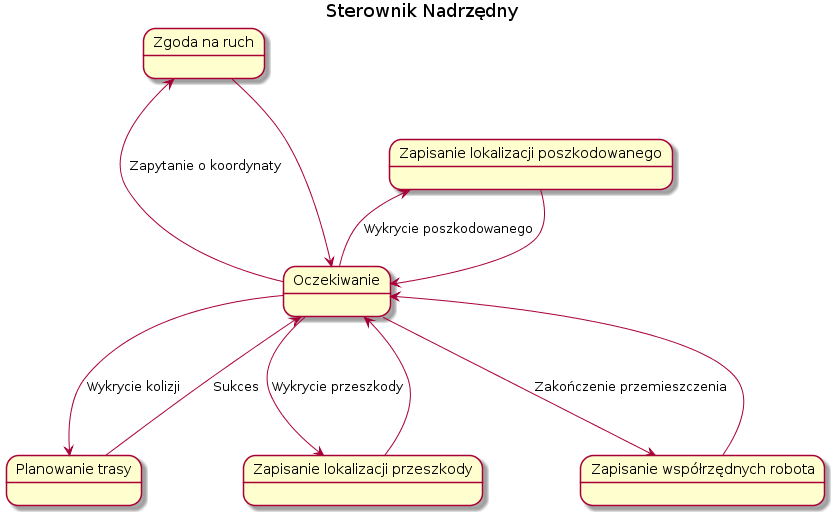
\includegraphics[width=1\textwidth]{gggg.png}
    \caption{Graf algorytmu sterownika nadrzędnego.}
    \label{fig:tiled}
\end{figure}
